\documentclass[12pt]{article}
\usepackage{../../format}
\lhead{A Level Physics}
\usepackage{enumitem}
\setcounter{secnumdepth}{4}
\usepackage{float}
\begin{document}
\begin{center}
\underline{\huge Paper 2 Cheat Sheet}
\end{center}
\section{Thermal physics}
\subsection{Thermal energy transfer}
\textbf{Specific heat capacity} - The energy required to raise the temperature of a unit mass of a given substance by one degree\\
\textbf{Specific latent heat}  - The energy required to change the state of a material without changing the temperature\\
\textbf{Temperature} - The average kinetic energy of the atoms or molecules in the system\\
\textbf{Heat} - Energy transfer due to a difference in temperature
\subsubsection{Continuous flow}
By dividing the specific heat capacity formula by t it can be found that
$$IV=mc\frac{\Delta T}{t}$$
This gives the power per second, where a mass $m$ flows in a time $t$
\subsection{Ideal gases}
{\renewcommand{\arraystretch}{2}
\begin{tabularx}{\textwidth}{|X|X|X|X|}
\hline
Law&Proportionality&Constant&Equation\\
\hline
Boyle's&$p\propto\dfrac{1}{v}$&Temperature, moles&$p_1v_1=p_2v_2$\\
\hline
Charles'&$V\propto T$&Pressure, moles&$\dfrac{v_1}{T_1}=\dfrac{v_2}{T_2}$\\
\hline
Gay-Lussac&$p\propto T$&Volume, moles&$\dfrac{p_1}{T_1}=\dfrac{p_2}{T_2}$\\
\hline
\end{tabularx}}
The two formulas on the formula book for the gas laws have $n$ moles and $N$ molecules
\subsubsection{Deriving Pressure volume work formula}
$$W=FS=F\times\Delta L=\frac{F}{A}\times A\Delta L=P\Delta V$$
\subsubsection{Types of masses}
\textbf{Molar mass} - The mass of a mole of a substance\\
\textbf{Molecular mass} - The mass of the molecules
\newpage
\subsection{Molecular kinetic theory model}
\subsubsection{Brownian motion as evidence for the existence of atoms}
\textbf{Brownian motion} - The random motion of smoke particles in a gas\\
As Newton's first law states that objects remain in motion until acted on by a force, the smoke particles should remain in motion, instead they move randomly, suggesting collisions with something else
\subsubsection{Explanation of relationships between p,V and T}
Increase pressure - More collisions, increase temperature. Same number of molecules, volume must decrease
\subsubsection{Empirical gas laws but theoretical kinetic theory}
By changing variables of a gas, the gas laws can be derived, however the kinetic theory is based on what else would be expected to be required to be constant.
\subsubsection{Derivation}
\textcolor{red}{Newton's $3^{\text{rd}}$ law - Every action has an equal and opposite reaction}\\
$\Delta mc=mc_{x1}--mc_{x1}=2mc_{x1}$\\
\\
\textcolor{red}{Use $\text{Velocity}=\dfrac{\text{Distance}}{\text{Time}}$}\\
Time=$\dfrac{\text{Distance}}{\text{Velocity}}=\dfrac{2l}{c_{x1}}$\\
\\
\textcolor{red}{Use force$=\dfrac{\text{Change in momentum}}{\text{time}}$}\\
$\text{Force}=\dfrac{\Delta mc}{\Delta t}=\dfrac{2mc{x1}}{2l/c_{x1}}=\dfrac{mc_{x1}^2}{l}$\\
\\
\textcolor{red}{Use Pressure$=\dfrac{\text{Force}}{\text{Area}}$}\\
\\
$p_1=\dfrac{mc_{x1}^2/l}{l^2}=\dfrac{mc_{x1}^2}{l^3}$\\
\\
\textcolor{red}{Expand for N particles}\\
$p=\Sigma p_n=p_1+p_2+p_3...+p_N$\\
\\
$p=\dfrac{mc_{x1}^2}{l^3}+\dfrac{mc_{x2}^2}{l^3}+\dfrac{mc_{x3}^2}{l^3}+\dfrac{mc_{xN}^2}{l^3}$\\
\\
$p=\dfrac{m}{l^3}(c_{x1}^2+c_{x2}^2+c_{x3}^2...+c_{xN}^2)$\\
\\
\textcolor{red}{The mean of all the squares of the velocities is written as $\mathlarger{\bar{c_x^2}}$}\\
\\
$\mathlarger{\bar{c_x^2}}=\dfrac{c_{x1}^2+c_{x2}^2+c_{x3}^2...+c_{xN}^2}{N}$\\
\\
$N\mathlarger{\bar{c_x^2}}=c_{x1}^2+c_{x2}^2+c_{x3}^2...+c_{xN}^2$\\
\\
\\
\textcolor{red}{Simplify expression for pressure}\\
$p=\dfrac{Nm\mathlarger{\bar{c_x^2}}}{l^3}$\\
\\
\textcolor{red}{Consider in 3 dimensions}\\
\\
$\mathlarger{\bar{c^2}=\bar{c_x^2}+\bar{c_y^2}+\bar{c_z^2}}$\\
\textcolor{red}{Average of mean square velocity for each dimension are equal}\\
\\
$\mathlarger{\bar{c_x^2}=\bar{c_y^2}=\bar{c_z^2}}$\\
\textcolor{red}{Simplify 3D formula}\\
\\
$\mathlarger{\dfrac{\bar{c^2}}{3}=\bar{c_x^2}=\bar{c_y^2}=\bar{c_z^2}}$\\
\\
\textcolor{red}{Simplify pressure formula}\\
\\
$p=\dfrac{1}{3}\times\dfrac{Nm\mathlarger{\bar{c^2}}}{l^3}$\\
\\
\textcolor{red}{Insert Density formula}\\
\\
$\rho=\dfrac{\text{Mass}}{\text{Volume}}=\dfrac{Nm}{l^3}$
\\
\textcolor{red}{Substitute into Pressure formula}\\
$$p=\frac{1}{3}\rho\mathlarger{\bar{c^2}}$$
\section{Fields and their consequences}
\subsection{Fields}
Similarities and differences between gravitational and electrostatic forces\\
\setitemize{noitemsep,topsep=-5pt,leftmargin=*}%Compress list
\begin{tabularx}{\textwidth}{|X|X|}
\hline
Similarities&Differences\\
\hline
\begin{itemize}
\item Inverse square laws
\item Use of field lines
\item Use of potential
\item Use of equipotentials
\end{itemize}& Masses always attract, but charges may attract or repel\\
\hline
\end{tabularx}
\newpage
\subsection{Gravitational fields}
\subsubsection{Gravitational field strength}
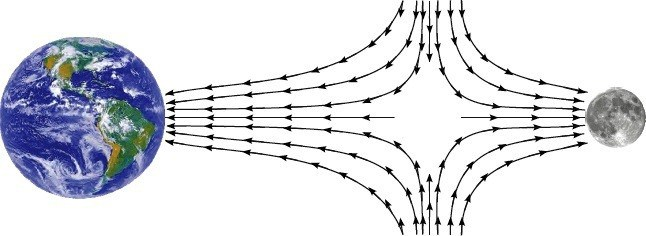
\includegraphics[width=8cm]{gravity.jpg}
\subsubsection{Gravitational potential}
Gravitational potential has a value of 0 at infinity, then reduces as it approaches the planet.\\
\textbf{Gravitational potential} - The work done in moving a unit mass from infinity to that point int he field\\
\textbf{Gravitational potential difference} - The work done in moving a unit mass from one point to another \\
\textbf{Equipotential} - The group of points with the same potential energy\\
\\
The sign is negative because a negative amount of work has to be done to move the object from infinity to earth because the object is attracted to earth.
\subsubsection{Orbits of planets and satellites}
\paragraph{Kepler's law}
$$F=\frac{GMm}{r^2}=\frac{mv^2}{r}\quad \therefore \frac{GM}{r}=v^2$$
$$v=\frac{s}{t}=\frac{2\pi r}{T}$$
$$v^2=\frac{4\pi^2r^2}{T^2}=\frac{GM}{r}$$
$$\frac{r^2}{T^2}=\frac{GM}{4\pi^2}$$
RHS is a constant
$$r^2\propto T^2$$
\paragraph{Escape velocity}
$$\frac{1}{2}mv^2=\frac{GMm}{r}\quad \therefore v=\sqrt{\frac{2GM}{r}}$$
$$g=\frac{GM}{r^2}\quad \therefore gr=\frac{GM}{r}$$
$$v=\sqrt{2gr}$$
\paragraph{Total energy of an orbiting satellite}
$$\textrm{Total energy=KE+GPE}$$
$$KE=\frac{1}{2}mv^2$$
$$\frac{GM}{r^2}=\frac{v^2}{r}\quad \therefore v^2=\frac{GM}{r}$$
$$KE=\frac{1}{2}m\frac{GM}{r}$$
$$GPE=mV \quad	V=-\frac{GM}{r} \quad \therefore E_p=-\frac{GMm}{r}$$
$$E_T=E_K+E_P=\frac{GMm}{2r}+-\frac{GMm}{r}=-\frac{GMm}{2r}$$
\paragraph{Synchronous orbits}
$ $\\
\textbf{Geosynchronous orbit} - Time period of 24h, will be seen at the same place at the same time every day\\ 
\textbf{Geostationary orbit} - Time period of 24h, but in the plane of the equator and travelling the same direction as the earth, appears stationary to an observer on the ground\\
\\
The height at which these satellites must be is determined by Kepler's law
\subsection{Electric fields}
\subsubsection{Coulomb's law}
This is the first equation under electric fields on the data sheet, it describes the force between two point charges in a vacuum\\
\textbf{Permittivity of free space} - The charge per unit area in coulombs per square metre on oppositely charged plates when the electric field strength between the plates is one volt per metre\\
The difference between the permittivity of free space and the permittivity of air is so insignificant air can be treated as a vacuum.\\
\textbf{Electric field strength} - At a point in an electric field, the force per unit charge on a small positively charged object in that field
\begin{center}
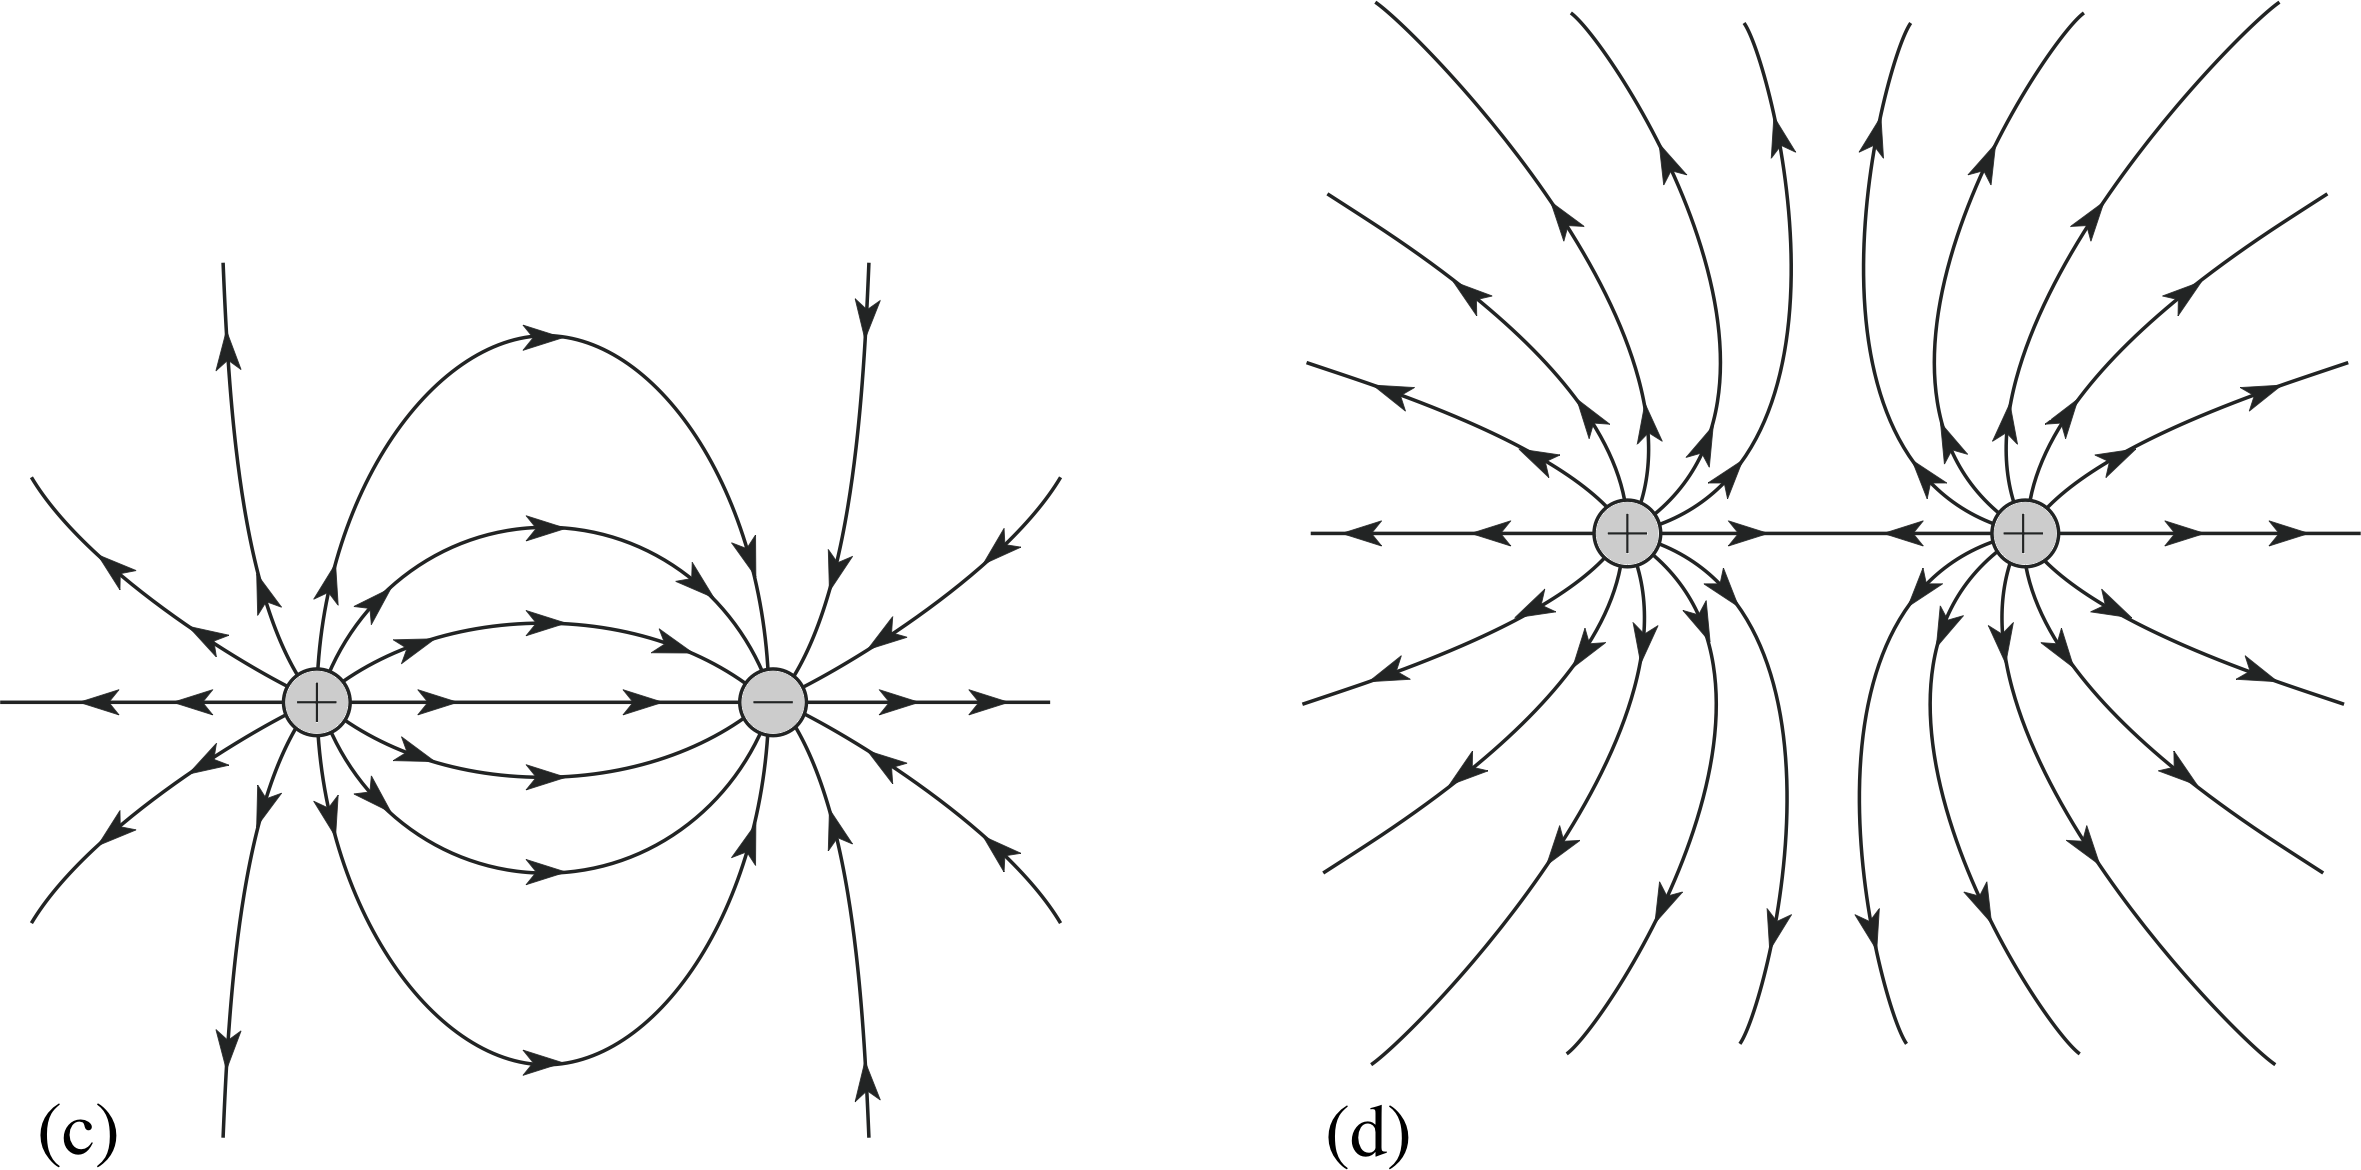
\includegraphics[width=12cm]{field_lines.png} 
\end{center}

\paragraph{Derive $Fd=Q\Delta V$}
$$F=EQ \quad E=\frac{V}{d} \quad\therefore F=\frac{QV}{d} \quad\therefore Fd=QV$$
\paragraph{Particle in a uniform electric field}
\begin{center}
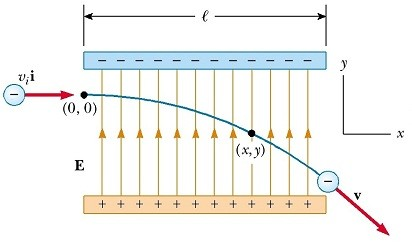
\includegraphics[width=8cm]{particle.jpg}
\end{center}
\subsubsection{Electric potential}
\textbf{Absolute electric potential} - At a point in an electric field, the work done per unit charge on a small positively charged object to move it from infinity to that point in the field
\subsection{Capacitance}
\subsubsection{Capacitance, parallel plate capacitor and energy stored in a capacitor}
\textbf{Capacitance} - The charge stored per unit p.d. of a capacitor\\
In the presence of an electric field, the polar molecules in the electric field will rotate, causing it to become polarised, and so a better dielectric. This is why polar molecules are used for dielectrics instead of non polar molecules
\subsubsection{Capacitor charge and discharge}
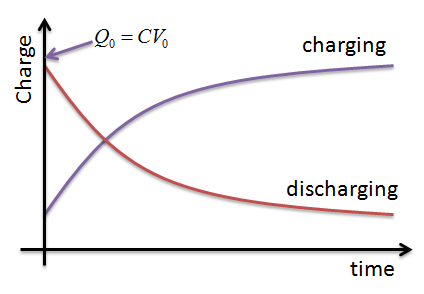
\includegraphics[width=6cm]{charge.png}
Voltage and charge follow the same pattern when charging and discharging, whereas current follows the opposite pattern.\\
The time constant(RC) is the time it until 37\% of the charge on the capacitor is remaining.
$$T_{\frac{1}{2}}=0.69RC$$
\subsection{Magnetic fields}
\subsubsection{Magnetic flux density}
\textbf{Magnetic flux density} - The magnetic force per unit length per unit current on a current carrying conductor at right angles to the field lines (Derive from F=BIl)
\subsubsection{Moving charges in a magnetic field}
$$F=BQv \quad \textrm{When the field is perpendicular to the velocity}$$
\paragraph{Cyclotron}
\begin{center}
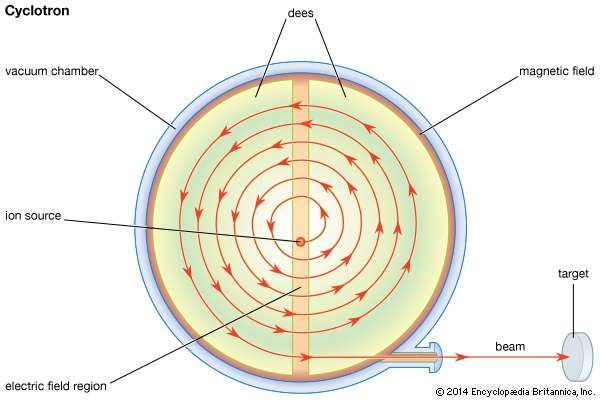
\includegraphics[width=10cm]{cyclotron.jpg}
\end{center}
This accelerates the particles to very high speeds, for use in medicine
\subsubsection{Magnetic flux and flux linkage}
$$\textrm{Magnetic flux:}\phi=BA \quad \textrm{Where B is normal to A}$$
\textbf{Flux} - $\phi=BA$ for a uniform magnetic field of flux density B that is perpendicular to an area A. Unit of Weber(Wb)\\
\textbf{Flux Linkage} - Through a coil of N turns, $N\phi=BAN\cos\theta$ where B is the magnetic flux density perpendicular to area A, unit also of Wb
\subsubsection{Electromagnetic induction}
\textbf{Faraday's law} - The induced emf in a circuit is equal to the rate of change of the magnetic flux linkage through the circuit\\
\textbf{Lenz's law} - When a current is induced in electromagnetic induction, the direction of the induced current is always such as to oppose the change that causes the current
\subsubsection{Alternating currents}
\textbf{Peak to peak} - The difference in the values between the two peak and the trough of an ac wave\\
\textbf{Root mean square} - The DC voltage that will give the same effect as the AC voltage
\paragraph{Oscilloscope}
$x$ axis - Time base\\
$y$ axis - Y sensitivity\\
The position and size of the waveform should be adjusted so that it takes up as much of the screen as possible, reducing uncertainty.
\subsubsection{Transformers}
\textbf{Eddy currents} - Induced currents in metal parts of ac machines\\
Inefficiencies:
\begin{itemize}
\item Eddy currents form in the metal core of the transformer, leading to a loss in power
\item Resistance in the windings around the transformer resulting in energy wasted as heat
\item Magnetisation and demagnetisation of the core causes loss in energy
\end{itemize}
Power is transmitted at high voltage in transmission lines so they can be at a low resistance, and as power dissipated is $I^2R$, the lower the current, the less power is wasted
\section{Nuclear physics}
\subsection{Radioactivity}
\subsubsection{Rutherford scattering}
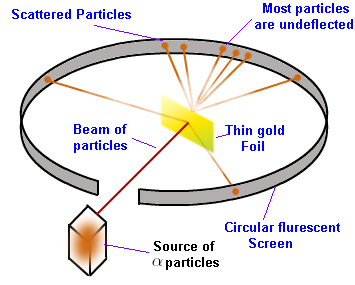
\includegraphics[width=8cm]{scatter.png}
Rutherford's experiment involved firing a beam of alpha particles at gold foil and measuring the paths of particles from the foil.
\begin{itemize}
\item Gold was used as it was expected to have a large nucleus
\item The screen fluoresces when collided with
\item This showed the atom was mostly empty space with a positive nucleus
\end{itemize}
\begin{figure}[H]
    \centering
    \begin{minipage}{0.45\textwidth}
        \centering
        
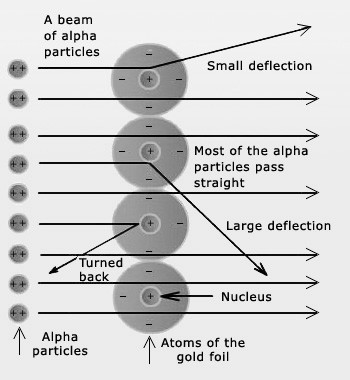
\includegraphics[width=6cm]{foil.jpg}  
    \end{minipage}\hfill
    \begin{minipage}{0.45\textwidth}
        \centering
\begin{tabularx}{\textwidth}{|X|X|}
\hline
Observation&Explanation\\
\hline
Most electrons pass all the way through&Atoms are mostly empty space\\
\hline
Some are deflected&The atom has a positive centre\\
\hline
Some are deflected by significant angles&The positive charge is condensed in a small area\\
\hline
\end{tabularx}
    \end{minipage}
\end{figure}
\subsubsection{$\alpha$, $\beta$ and $\gamma$ radiation}
\begin{tabularx}{\textwidth}{|c|X|X|X|}
\hline
&Alpha&Beta&Gamma\\
\hline
Nature&2 Protons+2 Neutrons&High speed electron or positron&High energy photon\\
\hline
Range&Up to 10cm&Up to 1m&Infinite\\
\hline 
Deflection in a magnetic field&Deflected&Opposite direction to $\alpha$ particles and more easily deflected&Not deflected\\
\hline
Absorption&Paper&Aluminium&Lead \\
\hline
Ionisation&$10^4$ ions per mm&100 ions per mm&Very weak ionising effect\\
\hline
Energy of each particle&Constant for a given source&Varies up to a maximum for a given source&Constant for a given source\\
\hline
\end{tabularx}
\paragraph{Inverse square law for gamma radiation}
$$I=\frac{k}{x^2}$$
\paragraph{Safety}$ $\\
Those working in areas of high radiation, for example nuclear power plants, should wear film badges which monitor a persons exposure to radiation
\paragraph{Background radiation}$ $\\
Background radiation has many sources:
\begin{itemize}
\item Air (Radon gas)
\item Medical
\item Ground and buildings
\item Food and drink
\end{itemize}
\paragraph{Uses of radiation in medicine}$ $\\
The health benefits from using radiation in medicine almost always outweigh the risks, but doctors must protect themselves as repeated exposure is dangerous
\end{document}